\documentclass[12pt]{article}

\usepackage[margin=1in]{geometry}
\usepackage{xcolor}
\usepackage{array}
\usepackage{booktabs}
\usepackage{tikz}
\usepackage{textcomp}
\usepackage{amsmath}
\usetikzlibrary{positioning,fit,backgrounds}

\definecolor{modelblue}{RGB}{52,120,246}
\definecolor{modelfill}{RGB}{227,238,255}
\definecolor{persongreen}{RGB}{34,139,34}
\definecolor{personfill}{RGB}{230,248,234}
\definecolor{dateorange}{RGB}{230,120,20}
\definecolor{datefill}{RGB}{255,239,220}
\definecolor{grayfill}{RGB}{245,245,245}
\definecolor{navyblue}{RGB}{25,25,112}

\begin{document}

\begin{center}
    {\LARGE \textbf{Entity Discovery and Type Induction Example}}
\end{center}

\vspace{0.5cm}

\section*{Input Text}

\noindent
\textbf{Sentence:} ``Transformer was introduced by Vaswani et al. in 2017.''

\vspace{0.6cm}

\section*{Possible Discovered Entities}

\begin{itemize}
    \item \fcolorbox{modelblue}{modelfill}{\strut Transformer}
    \item \fcolorbox{persongreen}{personfill}{\strut Vaswani}
    \item \fcolorbox{dateorange}{datefill}{\strut 2017}
\end{itemize}

\vspace{0.6cm}

\section*{Possible Induced Types}

\begin{center}
\renewcommand{\arraystretch}{1.4}
\begin{tabular}{lll}
\toprule
\textbf{Entity} & \textbf{Possible Type} & \textbf{Interpretation} \\
\midrule
Transformer & model / architecture & a technical method or system \\
Vaswani & researcher & a person name \\
2017 & year / date & a temporal expression \\
\bottomrule
\end{tabular}
\end{center}

\vspace{0.8cm}

\section*{Inline Visualization}

\begin{center}
\fcolorbox{modelblue}{modelfill}{\strut Transformer}
\hspace{0.3em}
$\rightarrow$
\hspace{0.3em}
\texttt{model / architecture}

\vspace{0.4cm}

\fcolorbox{persongreen}{personfill}{\strut Vaswani}
\hspace{0.3em}
$\rightarrow$
\hspace{0.3em}
\texttt{researcher}

\vspace{0.4cm}

\fcolorbox{dateorange}{datefill}{\strut 2017}
\hspace{0.3em}
$\rightarrow$
\hspace{0.3em}
\texttt{year / date}
\end{center}

\vspace{0.8cm}

\section*{Sentence-Level Visualization}

\begin{center}
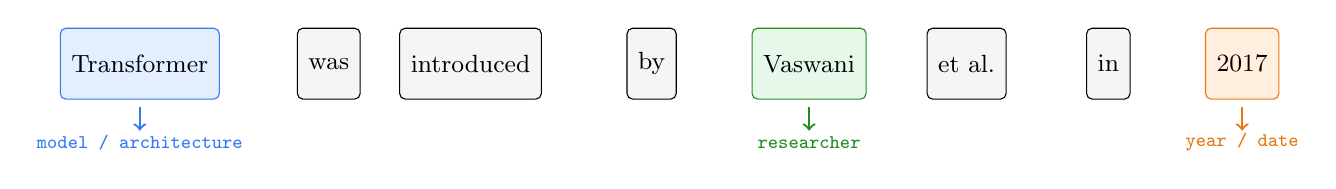
\begin{tikzpicture}[
    token/.style={draw, rounded corners=2pt, minimum height=0.9cm, align=center, font=\small, inner sep=4pt},
    labelstyle/.style={font=\scriptsize\ttfamily}
]

\node[token, fill=modelfill, draw=modelblue] (t1) at (0,0) {Transformer};
\node[token, fill=grayfill] (t2) at (2.4,0) {was};
\node[token, fill=grayfill] (t3) at (4.2,0) {introduced};
\node[token, fill=grayfill] (t4) at (6.5,0) {by};
\node[token, fill=personfill, draw=persongreen] (t5) at (8.5,0) {Vaswani};
\node[token, fill=grayfill] (t6) at (10.5,0) {et al.};
\node[token, fill=grayfill] (t7) at (12.3,0) {in};
\node[token, fill=datefill, draw=dateorange] (t8) at (14.0,0) {2017};

\node[labelstyle, text=modelblue] at (0,-1.0) {model / architecture};
\node[labelstyle, text=persongreen] at (8.5,-1.0) {researcher};
\node[labelstyle, text=dateorange] at (14.0,-1.0) {year / date};

\draw[->, thick, modelblue] (0,-0.55) -- (0,-0.85);
\draw[->, thick, persongreen] (8.5,-0.55) -- (8.5,-0.85);
\draw[->, thick, dateorange] (14.0,-0.55) -- (14.0,-0.85);

\end{tikzpicture}
\end{center}

\vspace{0.8cm}

\section*{Compact Thesis-Friendly Version}

\noindent
For example, given the sentence ``Transformer was introduced by Vaswani et al. in 2017,'' an entity discovery module may identify \textit{Transformer}, \textit{Vaswani}, and \textit{2017} as salient spans. A type induction module may then assign them the semantic types \texttt{model / architecture}, \texttt{researcher}, and \texttt{year / date}, respectively.

\end{document}